 \documentclass[9pt, final]{beamer}\usepackage[]{graphicx}\usepackage[]{color}
%% maxwidth is the original width if it is less than linewidth
%% otherwise use linewidth (to make sure the graphics do not exceed the margin)
\makeatletter
\def\maxwidth{ %
  \ifdim\Gin@nat@width>\linewidth
    \linewidth
  \else
    \Gin@nat@width
  \fi
}
\makeatother

\definecolor{fgcolor}{rgb}{0.345, 0.345, 0.345}
\newcommand{\hlnum}[1]{\textcolor[rgb]{0.686,0.059,0.569}{#1}}%
\newcommand{\hlstr}[1]{\textcolor[rgb]{0.192,0.494,0.8}{#1}}%
\newcommand{\hlcom}[1]{\textcolor[rgb]{0.678,0.584,0.686}{\textit{#1}}}%
\newcommand{\hlopt}[1]{\textcolor[rgb]{0,0,0}{#1}}%
\newcommand{\hlstd}[1]{\textcolor[rgb]{0.345,0.345,0.345}{#1}}%
\newcommand{\hlkwa}[1]{\textcolor[rgb]{0.161,0.373,0.58}{\textbf{#1}}}%
\newcommand{\hlkwb}[1]{\textcolor[rgb]{0.69,0.353,0.396}{#1}}%
\newcommand{\hlkwc}[1]{\textcolor[rgb]{0.333,0.667,0.333}{#1}}%
\newcommand{\hlkwd}[1]{\textcolor[rgb]{0.737,0.353,0.396}{\textbf{#1}}}%
\let\hlipl\hlkwb

\usepackage{framed}
\makeatletter
\newenvironment{kframe}{%
 \def\at@end@of@kframe{}%
 \ifinner\ifhmode%
  \def\at@end@of@kframe{\end{minipage}}%
  \begin{minipage}{\columnwidth}%
 \fi\fi%
 \def\FrameCommand##1{\hskip\@totalleftmargin \hskip-\fboxsep
 \colorbox{shadecolor}{##1}\hskip-\fboxsep
     % There is no \\@totalrightmargin, so:
     \hskip-\linewidth \hskip-\@totalleftmargin \hskip\columnwidth}%
 \MakeFramed {\advance\hsize-\width
   \@totalleftmargin\z@ \linewidth\hsize
   \@setminipage}}%
 {\par\unskip\endMakeFramed%
 \at@end@of@kframe}
\makeatother

\definecolor{shadecolor}{rgb}{.97, .97, .97}
\definecolor{messagecolor}{rgb}{0, 0, 0}
\definecolor{warningcolor}{rgb}{1, 0, 1}
\definecolor{errorcolor}{rgb}{1, 0, 0}
\newenvironment{knitrout}{}{} % an empty environment to be redefined in TeX

\usepackage{alltt}
  \mode<presentation>{\usetheme{rml}}
  % \usepackage[english]{babel}
  \usepackage[latin1]{inputenc}
  % \usepackage{grffile}
  \usepackage{graphics}
  \usepackage{amsmath, amsthm, amssymb, latexsym, xcolor}
  \usepackage{pgf, tikz}
  \usetikzlibrary{arrows, matrix, positioning}
  %\usepackage{times}\usefonttheme{professionalfonts}
  
  \usepackage{mathpazo} % Palatino
  % \usepackage{avant}    % Avant Garde
  % \renewcommand{\familydefault}{\rmdefault}
  
  \usefonttheme[]{serif}
  % \boldmath
  \usepackage[orientation=portrait, size=a0, scale=1.3, grid, debug]{beamerposter}               
    \usepackage{array, booktabs, tabularx}
    \newcolumntype{Z}{>{\centering\arraybackslash}X} % centered tabularx columns
    \newcommand{\pphantom}{\textcolor{ta3aluminium}} % phantom introduces a vertical space in p formatted table columns??!!  
  
  \title{Multimatrix Extension of Partial Least Square}
  \author{\small Raju Rimal (Supervisor: Solve S{\ae}bo, Trygve Alm{\o}y)}
  \institute[Norwegian University of Life Sciences (NMBU)]{\footnotesize Norwegian University of Life Sciences (NMBU), {\AA}s, Norway}
  \date[15 August, 2015]{15 August, 2015}
  
%%%%%%%%%%%%%%%%%%%%%%%%%%%%%%%%%%%%%%%%%%%%%%%%%%%%%%%%%%%%%%%%%%%%%%%%%%%%%%%%%%%%%%
\newlength{\topcolumn}
\setlength{\topcolumn}{0.49\textheight}
\newlength{\bottomcolumn}
\setlength{\bottomcolumn}{0.51\textheight}
%%%%%%%%%%%%%%%%%%%%%%%%%%%%%%%%%%%%%%%%%%%%%%%%%%%%%%%%%%%%%%%%%%%%%%%%%%%%%%%%%%%%%%

\usepackage[backend=bibtex,  natbib=true]{biblatex}
\addbibresource{references.bib}
\renewcommand\bibfont{\small}
\setbeamercolor*{bibliography entry title}{fg=black}
\setbeamercolor*{bibliography entry author}{fg=black}
\setbeamercolor*{bibliography entry location}{fg=black}
\setbeamercolor*{bibliography entry note}{fg=black}
\setbeamertemplate{bibliography item}[text]
\IfFileExists{upquote.sty}{\usepackage{upquote}}{}
\begin{document}
\begin{frame}[fragile]




% !Rnw root = main.Rnw
\begin{columns}
    % ---------------------------------------------------------%
    % Set up a column 

% !Rnw root = main.Rnw
\begin{column}{.49\textwidth}
      \begin{beamercolorbox}[center, wd=\textwidth]{postercolumn}
        \begin{minipage}[T]{.98\textwidth}  % tweaks the width, makes a new \textwidth
          \parbox[t][\topcolumn]{\textwidth}{ % must be some better way to set the the height, width and textwidth simultaneo3usly
            % Since all columns are the same length, it is all nice and tidy.  You have to get the height empirically
            % ---------------------------------------------------------%
            
            % fill each column with content            
            \begin{block}{Partial Least Square Regression} % Introduction Block
            Lets consider a model with multiple response \textbf{Y}, predictor matrix \textbf{X} and error matrix \textbf{E} as,
            \[ \mathbold{Y} = \boldsymbol{B}_\circ + \mathbold{XB} + \boldsymbol{E} \]            
			\begin{columns}[t, onlytextwidth]
				\column{0.34\textwidth}
				\textbf{Usual Problems}\\
					\begin{itemize}
						\item Multicollinear Predictors
						\item High Dimensional dataset
						\item Large Number of predictors
					\end{itemize}
				\column{0.64\textwidth}
				\textbf{Partial Least Square Regression}\\
					Partial Least Square (PLS) regression is a method that can,
					\begin{itemize}
						\item explore the underlying predictor-response relationship through latent structures
						\item capture maximum covariance structure between \textbf{X} and \textbf{Y} in first few principle components
					\end{itemize}
			\end{columns}
			\vspace{1cm}
            \begin{columns}[b]
              \begin{column}{0.45\textwidth}
                \begin{figure}
                \centering
                  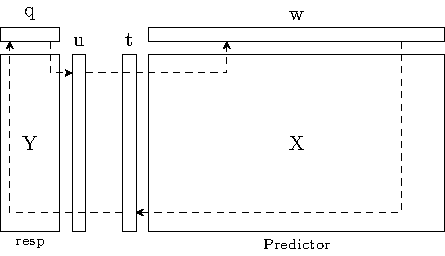
\includegraphics[width = 0.9\textwidth]{figure/plsr}
                  \caption{NIPALS algorithm for performing PLS regression. Starting from any arbitrary column \textbf{u}, the algorithm converges after few loops. For each required components, the algorithm creates loadings and scores for \textbf{X} and \textbf{Y} with coefficients estimates. After extraction of each component, the \textbf{X} and \textbf{Y} matrices are deflated ensuring that the components obtained are independent to each other.}
                  \label{fig:pls}
                \end{figure}
	           \end{column} 
              \begin{column}{0.45\textwidth}
              		\begin{exampleblock}{PLS Algorithm}
           			\begin{align*}
           				\mathtt{[X0, Y0]} & \leftarrow \mathtt{scale(X, Y)} \\
           				\mathtt{w} & \leftarrow \texttt{Obtained from}\\
           				& \texttt{\; \; \;NIPALS algorithm} \\
           				\mathtt{w} & \leftarrow \mathtt{w/|w|} \\
           				\mathtt{t} & \leftarrow \mathtt{X_0w} \\
           				\mathtt{p} & \leftarrow \mathtt{X_a^tt(t't)^{-1}}\\
           				\mathtt{q} & \leftarrow \mathtt{Y_a^tt(t't)^{-1}}
              	\end{align*}	
              		\texttt{--- Deflation ---}
              	\begin{align*}
              		\mathtt{X_{a+1}} & \leftarrow \mathtt{X_a - tp^t} \\
             			\mathtt{Y_{a+1}} & \leftarrow \mathtt{Y_a - tq^t} 
	             	\end{align*}	
           			\texttt{---  Coefficients Estimate ---}
             		\[\mathtt{\hat{\mathbf{B}}} \leftarrow \mathtt{\mathbf{W(P^tW)^{-1}Q}}\]
              		\end{exampleblock}
         \end{column}% End of Column: NIPALS Algorithm
            %% -----------------------------------------------%%  
            \end{columns} % End of PLS upper columns
            %% -----------------------------------------------%%
            \end{block}
            \begin{block}{References}
            \nocite{Martens:2005aa, wold2001pls,saebo2010three, saebo2015Academia}
            {\printbibliography}
            \end{block}
            
}
        \end{minipage}
      \end{beamercolorbox}
\end{column}
    % ---------------------------------------------------------%
    % end the column
    
    % ---------------------------------------------------------%
    % Set up a column 

% !Rnw root = main.Rnw
\begin{column}{.49\textwidth}
      \begin{beamercolorbox}[center,wd=\textwidth]{postercolumn}
        % tweaks the width, makes a new \textwidth
        \begin{minipage}[T]{.98\textwidth} 
          \parbox[t][\topcolumn]{\textwidth}{ 
          % must be some better way to set the the height, 
          % width and textwidth simultaneously
          % Since all columns are the same length, it is all nice and tidy.  
          % You have to get the height empirically
          % ---------------------------------------------------------%
          % fill each column with content
            \begin{block}{L-PLS and its variants (Exo-LPLS and Endo-LPLS)} % Visulazation block
            	\begin{columns}[b]
            		\begin{column}{0.35\textwidth}
            			\begin{figure}
            				\centering
            				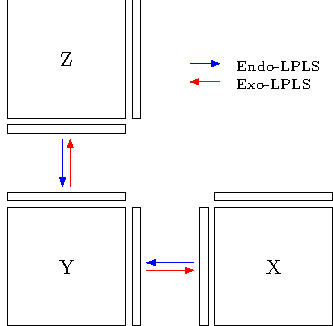
\includegraphics[width = \textwidth]{figure/lpls}
            				\caption{Extension of PLS including some background information}
            				\label{fig:lpls}
            			\end{figure}
            		\end{column}
            		\begin{column}{0.63\textwidth}
            			\begin{itemize}
            				\item Partial Least Square can also be used in understanding the covariance structure and the relation between different matrices. 
            				\item More information can give better insight in solving any problem. So, a background information on variation under study helps to model the complex dynamics of the real world phenomena.
            				\item L-shaped PLS (LPLS) helps in exploring covariance structure of three matrices.
            				\item LPLS with its variant Endo and Exo LPLS, enables to see the relationship between two matrices with no direct connection.
            			\end{itemize}
            		\end{column}
            	\end{columns}            
            	
            	
            \end{block}
            \vfill
            \begin{block}{U-shaped Partial Least Square Regression (UPLS)}
            	\begin{columns}[T, onlytextwidth]
            		\column{0.34\textwidth}
	            		\begin{figure}[H]
		            	\centering
             			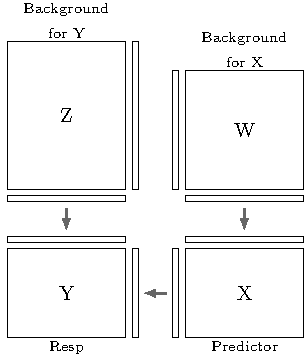
\includegraphics[width = \textwidth]{figure/upls}
             			\caption{UPLS structure}
             			\label{fig:upls}
	            		\end{figure}
             		\column{0.6\textwidth}
			            \begin{description}
			            \item[\textbf{Scenario}]\hfill\\
			            \begin{itemize}
			            	\item Large amount of chaotic yet informative data streams, if organized, can give light on any research process
			            	\item Integration of such easily available data source can supply background information to the variables under study and helps, not only to understand the causal relationship and covariance structure, but also to visualize them in understandable form and generate new hypothesis
			            \end{itemize}
				        \end{description}
				\end{columns}  
				\vspace{1cm}      
				\begin{description}
					\item[\textbf{What is UPLS}]\hfill\\
					UPLS is an extension of LPLS that enable us to,
					\begin{itemize}
						\item include background information for predictor matrix \textbf{X} and response matrix \textbf{Y}
						\item Foresee the relationship between two matrices that are from entirely different situations, i.e. the relation between \textbf{W} and \textbf{Z} through the eye of \textbf{X} and \textbf{Y} (Figure above)
					\end{itemize}
				\end{description}
            \end{block}
          }
          % ---------------------------------------------------------%
          % end the column
        \end{minipage}
      \end{beamercolorbox}
\end{column}

    % ---------------------------------------------------------%
    % end the column
\end{columns}
\vspace{1cm}
\begin{columns}
\begin{column}{\textwidth}
\begin{beamercolorbox}[center, wd=\textwidth]{postercolumn}
  \begin{minipage}[T]{0.98\textwidth}  % tweaks the width, makes a new \textwidth
    \parbox[t][\bottomcolumn]{\textwidth}{ 
      % ---------------------------------------------------------%
      
      % fill each column with content            
\begin{block}{Application Example}
\begin{columns}[T, onlytextwidth]
\begin{column}{0.34\textwidth}
\begin{description}
\item[\textbf{Hypothesis}]\hfill\\
	\begin{itemize}
		\item The personality-type of students have influence on their performance. 
		\item The better/poor score in a course of a student may be due to the inappropriate choice of teaching methods which does not correspond to their personality-types.
	\end{itemize}
	\vspace{1cm}
\item[\textbf{Materials}]\hfill\\
	\begin{itemize}
		\item Personality test data for 50 variables from 288 students through questionnaire (\textbf{X})
		\item Scores of 50 students in 9 courses constitute matrix \textbf{Y}
		\item Personality test data (\textbf{W}) for 2200 persons from various fields are used as background information for \textbf{X}
		\item Scores of 5000 students in the same 9 courses are also included as background information for \textbf{Y}
	\end{itemize}
	\vspace{1cm}
\item[\textbf{Missing Value Problem}]\hfill\\
	All the student considered have not taken all the 9 courses which creates lots of missing values. Following approaches are intended to apply,
	\begin{itemize}
		\item Ignore the missing observations within the NIPALS loop
		\item Replacing the missing value through interpolation or with nearest neighbor
	\end{itemize}
\end{description}
\end{column}
\begin{column}{0.62\textwidth}
\begin{figure}
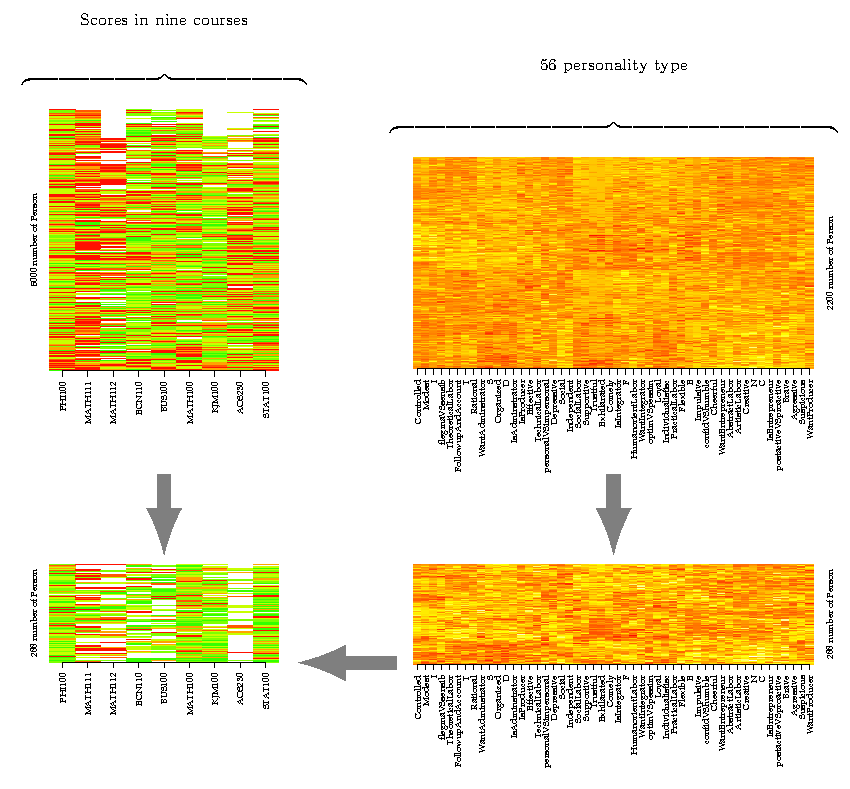
\includegraphics[width = \textwidth]{figure/application}
\end{figure}
\end{column}
\end{columns}
\end{block}
}
\end{minipage}
\end{beamercolorbox}
\end{column}
\end{columns}
\end{frame}
\end{document}
